\chapter{Search}

\section{Search Problems}

Searching is one of the most \itblue{fundemental techniques} in AI, underlying sub-module in many AI systems. Ai can \itblue{solve} many problems that homansare not good at, and achieve \itblue{super-human performance} in many domains (e.g. chess, go, etc.).

\begin{listu}
    \item \textbf{Benefits}

    \begin{listu}
        \item Useful as ageneral algorithmic technique for solving problems, both in AI and in other areas.

        \item Outperform humans in some areas (e.g. games). 

        \item Practical:

        \begin{listu}
            \item Many problems don't have specific algorithms for solving them.
            \item Useful in approximation (e.g., local search in optimization problems).
        \end{listu}

        \item Some critical aspects of intelligent behaviour, e.g., planning, can be cast as search.
    \end{listu}
    
    \item \textbf{Limitations}
    
    \begin{listu}
        \item Only shows how to solve the problem once we have it correctly formulated.
    \end{listu}
\end{listu}

% TODO: Planning and Scheduling Problems:

\subsection{Formalizing a Problem as a Search Problem}

\begin{listu}
    \item Necessary components
    
    \begin{listo}
        \item \bred{State Space}: A \term{state} is a representation of a \itblue{configuration} of the problem domain. The state space is the \itblue{set of all states} include in our model of the problem. 
        \item \bred{Initial State}: The starting configuration. 
        \item \bred{Goal State}: The configuration one wants to achieve. 
        \item \bred{Actions} (or State Space Transitions): Allowed changed to move from one state to another. 
    \end{listo}

    \item Optional Ingredients 
    
    \begin{listu}
        \item \itblue{Costs}: Representing the cost of moving from state to state. 
        \item \itblue{Heuristics}: Help guide the search process. 
    \end{listu}
\end{listu}

Once a search problem is formalized, there are a number of algorithms one can use to solve it. A \term{solution} is a \itblue{sequence of actions} or moves that can transform the \bred{initial state} into a \bred{goal state}. 

\begin{example}[Romania Travel]
    We want to travel in Romania from Arad to Bucharest as fast as possible. 

    \begin{center}
        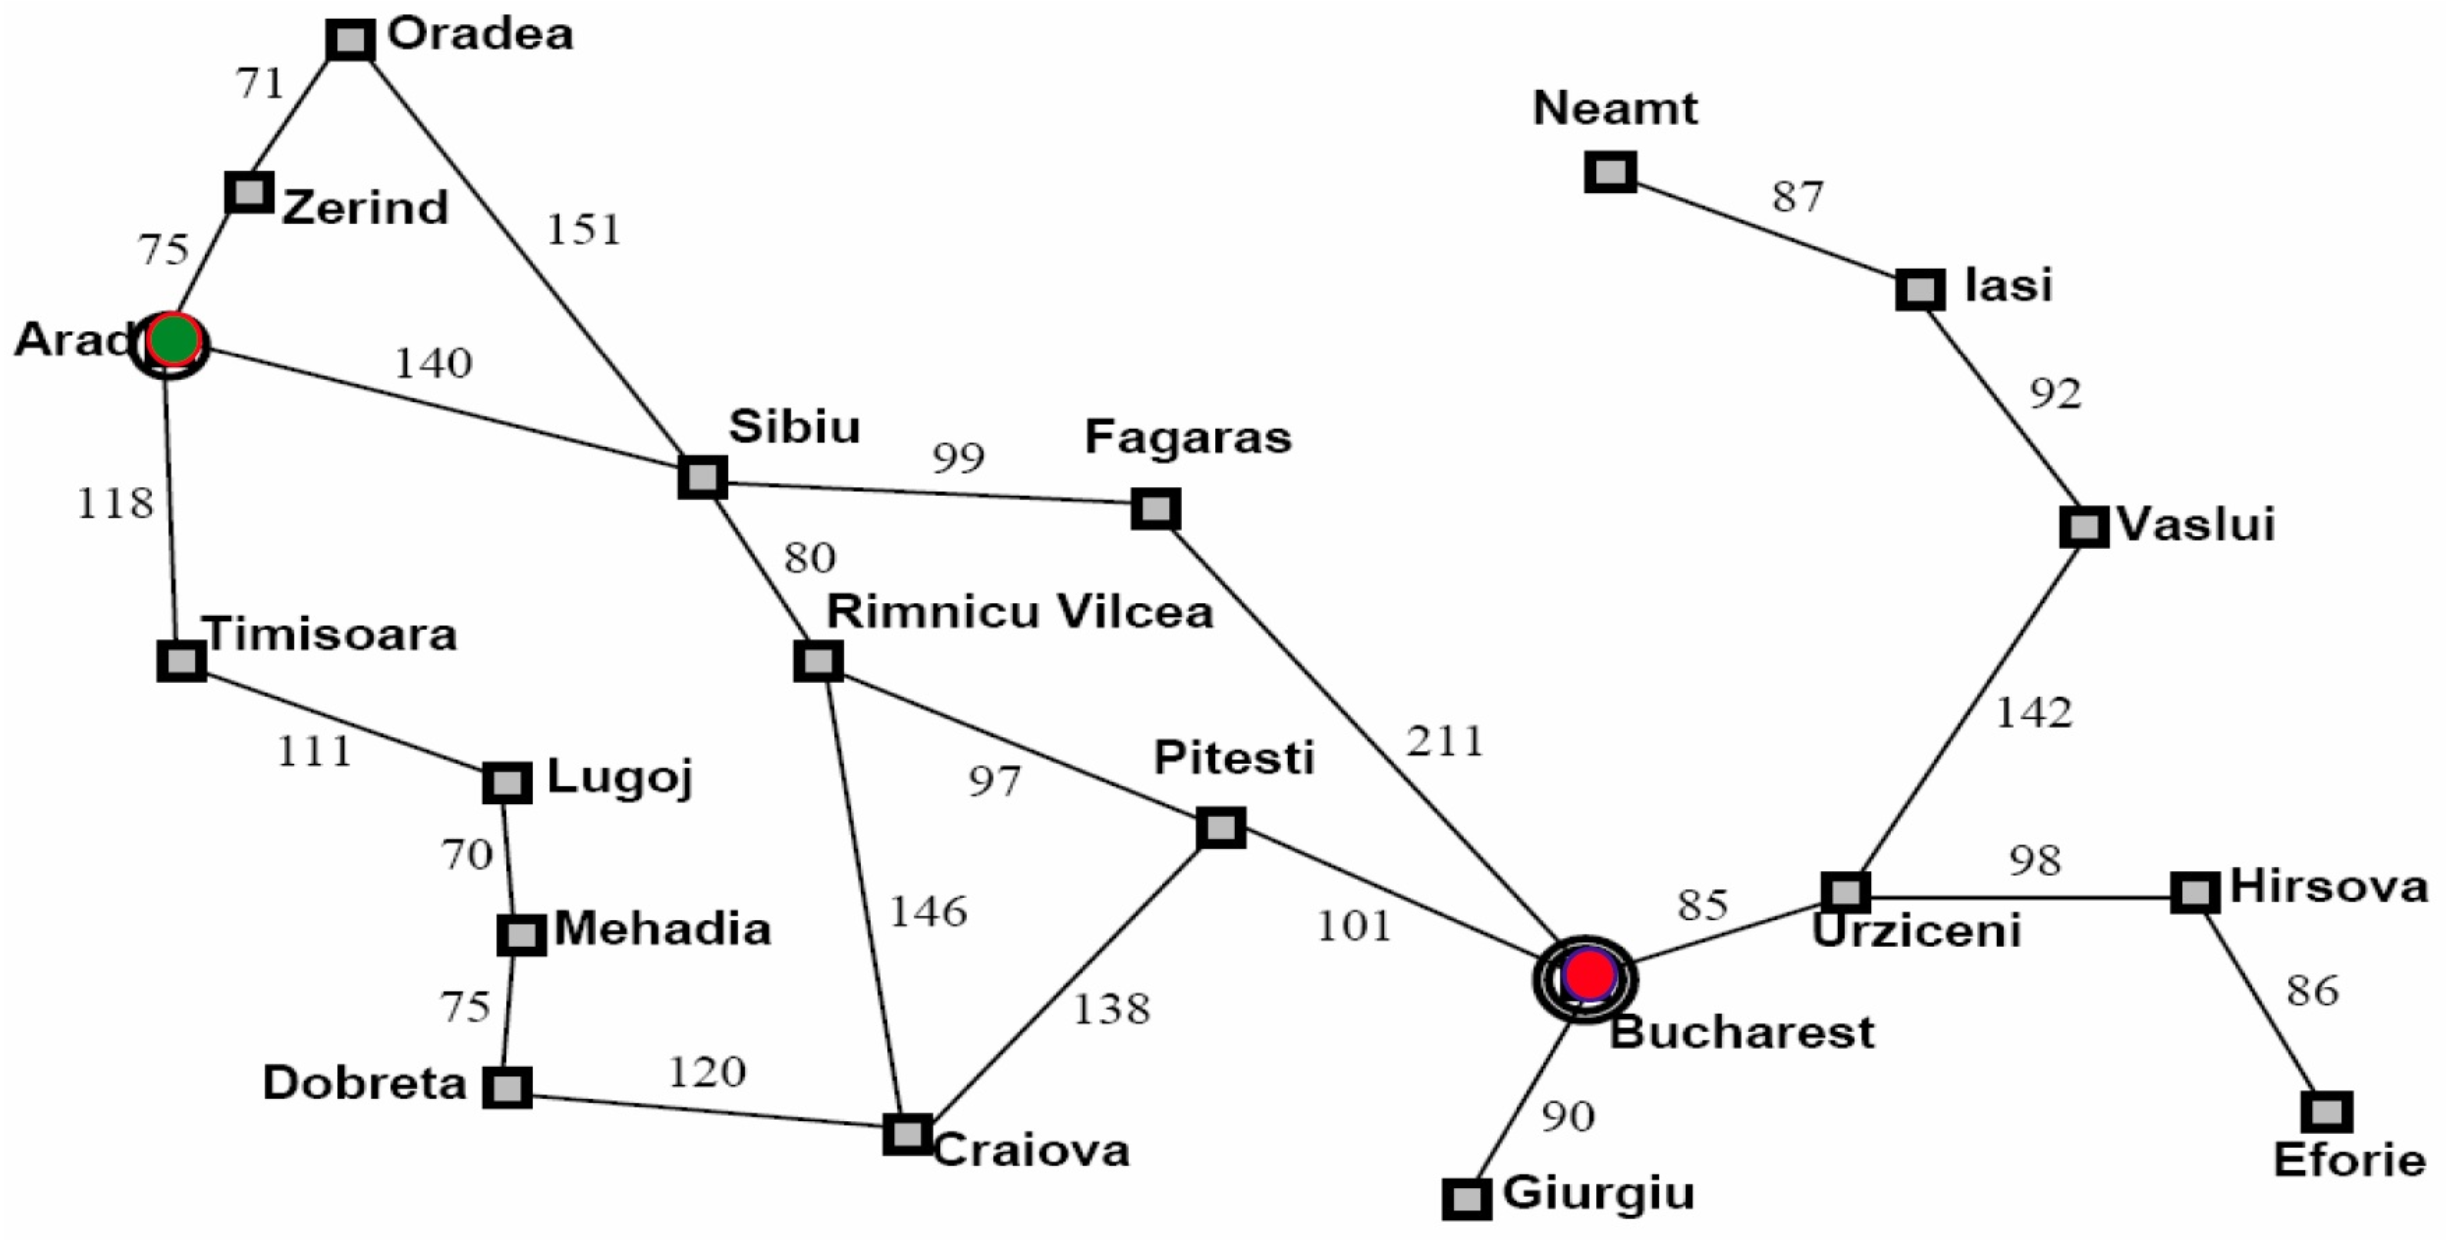
\includegraphics[width=0.75\linewidth]{figures/Romania Travel.png}
    \end{center}

    Each state would be a city. 

    \begin{listu}
        \item \bred{State Space}: The set of all cities on the map.
        \item \bred{Initial State}: Arad.
        \item \bred{Goal State}: Bucharest.
        \item \bred{Actions}: Driving between neighbouring cities.
    \end{listu}
\end{example}

\begin{example}[Water Jugs]
    We have a 3-liter jug and a 4-liter jug. We can fill either jug to the top from a tap, or we can empty either jug onto the ground. We can also pour the contents of one jug into the other until the receiving jug is full or the pouring jug is empty.

    Suppose initially the 4-liter jug is full, we want to have exactly 2 liters in the 3-liter jug.

    {~~~}

    We can use a pair of numbers to represent the state of the system: the amount of water in the 3-liter jug and the amount of water in the 4-liter jug.

    \begin{listu}
        \item \bred{State Space}: The set of all pairs of numbers $(a, b)$ where $a$ is the amount of water in the 3-liter jug and $b$ is the amount of water in the 4-liter jug.
        \item \bred{Initial State}: $(0, 4)$.
        \item \bred{Goal State}: $(2, 0)$, $(2, 1)$, $(2, 2)$, $(2, 3)$, $(2, 4)$.
        \item \bred{Actions}: 
        \begin{listu}
            \item Fill the 3-liter jug from the tap.
            \item Fill the 4-liter jug from the tap.
            \item Empty the 3-liter jug onto the ground.
            \item Empty the 4-liter jug onto the ground.
            \item Pour the contents of the 3-liter jug into the 4-liter jug.
            \item Pour the contents of the 4-liter jug into the 3-liter jug.
        \end{listu}
    \end{listu}

    \begin{remark}
        When formalizing a search problem, always consider these questions:

        \begin{listo}
            \item Can we reach all states fron any given start state?

            \item Will all actions result in a change of state? 

            \bred{No!} Imagine you have $(3, 4)$ and you try to fill the 3-liter jug from the tap. You will still have $(3, 4)$.
        \end{listo}
    \end{remark}
\end{example}

% \subsubsection{More Complex Situations}

In more complex situations, 

\begin{listu}
    \item Actions may lead to \bred{multiple states}. 
    
    For example, filpping a coin may lead to heads or tails.

    \item We may not be \bred{sure of a given state}
    
    For example, when prize is behind door 1, 2, or 3.

    \item Such situations require techniques for reasoning under uncertainty: assign probabilities to given outcomes.
\end{listu}

\subsection{Graphical Representation}

\begin{center}
    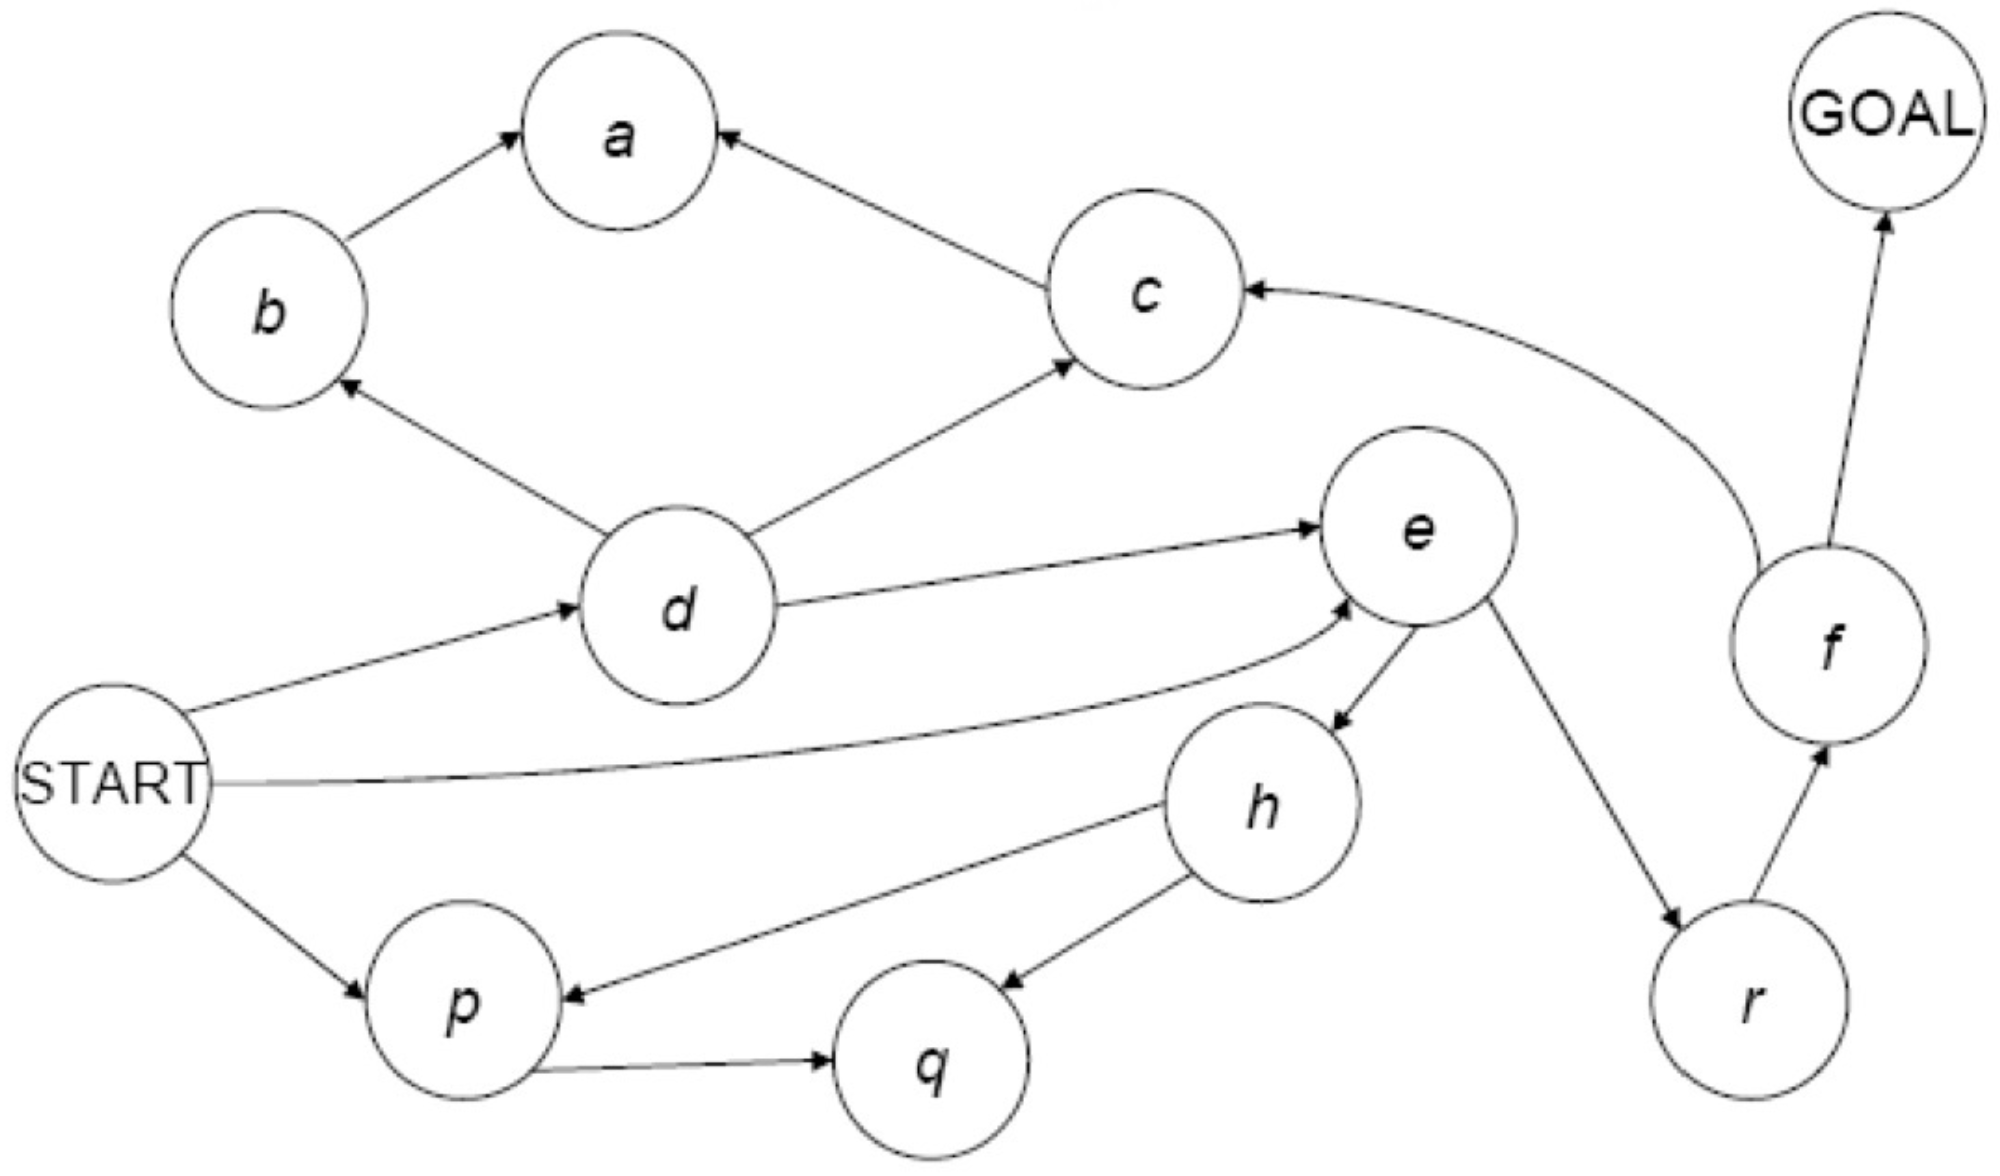
\includegraphics[width=0.5\linewidth]{figures/Search Graph Rep.png}
\end{center}

Assuming a finite search space, the

\begin{listu}
    \item \bred{vertices} represent states in the search space; and the 
    \item \bred{edges} represent transitions resulting from actions (or successor functions).
\end{listu}

\subsubsection{Search Tree}

\begin{definition}[Search Tree]
    A \term{search tree} is a \itblue{directed graph} where

    \begin{listu}
        \item Each node represents a state.
        \item Each edge represents an action.
        \item The root node represents the initial state.
        \item The leaf nodes represent goal states.
    \end{listu} 
\end{definition}

A search tree reflects the behaviour of an algorithm as it walks through a search problem. It has two important properties:

\begin{listu}
    \item \term{Solution depth}, denoted $d$, the depth of the shallowest goal node in the tree.
    \item \term{Maximum branching factor}, denoted $b$, the maximum number of children of any node in the tree.
\end{listu}

\begin{remark}
    Note that the \bred{same} state may appear \bred{multiple times} in a search tree.
\end{remark}

\begin{remark}
    It is important to distinguish between \bred{states} from \bred{nodes}. 

    \begin{listu}
        \item A \bred{state} represents a possible configuration of the world. 
        \item A \itblue{node} is a data structure constituting part of a search tree. It includes 
        \begin{listu}
            \item a \bred{state} and 
            \item the \bred{parent node}, 
            \item the \bred{action} that led to this node, and 
            \item the \bred{cost} of the path from the initial node to this node. 
        \end{listu}
        \item  Intuitively speaking, each node corresponds with a path from the initial state to the node's state.
        \item Two \bred{different nodes} are allowed to contain the \bred{same world state}.
    \end{listu}
\end{remark}

\subsection{Algorithms for Search}

\begin{listu}
    \item \textbf{Input}
    
    \begin{listu}
        \item \textbf{Initial node}

        \item \textbf{Successor Function} $S(x)$
        
        returns the set of nodes that can be reached from node $c$ via a single action. 

        \item \textbf{Goal Test Function} $G(x)$
        
        returns true if node $c$ satisfies the goal condition. 

        \item \textbf{Action Cost Function} $C(x, a, y)$
        
        returns the cost of moving from node $x$ to node $y$ using action $a$.

        Note that $C(x, a, y) = \infty$ if $y$ is not reachable from $a$ via $a$. 
    \end{listu}

    \item \textbf{Output}
    
    \begin{listu}
        \item A \itblue{sequence of actions} that transforms the initial node satisfying the goal test. 
        \item The sequence might be, \term{optimal in cost} for some algorithms, \term{optimal in length} for some algorithms, come with \bred{no optimality} guarantees from other algorithms.
    \end{listu}

    \item \textbf{Procedure}
    
    \begin{listu}
        \item Put nodes have not yet expanded in a list called the \term{\Frontier} (or \term{Open}).
        \item Initially, only the \itblue{initial node} is in the \Frontier.
        \item At each iteration, pull a node from the \Frontier, apply $S(x)$, and insert the children back into the \Frontier.
        \item Repeat until pulling a goal node.
    \end{listu}
\end{listu}

% \newpage
\begin{algorithm}
    \caption{Tree Search Algorithm}
    
    \begin{algorithmic}[1]
        \Function{Tree-Search}{Frontier, Successors, Goal?}
            % If frontier is empty, return failure
            \If{Frontier is empty}
                \State \Return failure
            \EndIf

            \State Curr $\gets$ select state from frontier

            \If{Goal?(Curr)}
                \State \Return Curr
            \EndIf

            \State Frontier' $\gets$ (Frontier $-$ \{ Curr \}) $\cup$ Successors(Curr)

            \State \Return \Call{TreeSearch}{Frontier', Successors, Goal?}
        \EndFunction
    \end{algorithmic}
\end{algorithm}

% TODO: example

Note that the search terminates only when a goal node is expanded into the \Frontier.

\subsubsection{Critical Properties of Search}

\begin{listu}
    \item \textbf{Completeness}
    
    \begin{listu}
        \item A search algorithm is \term{complete} if it always finds a solution if one exists.
    \end{listu}

    \item \textbf{Optimality}
    
    \begin{listu}
        \item A search algorithm is \term{optimal} if it always finds a solution with the lowest cost.
    \end{listu}

    \item \textbf{Time Complexity}
    
    \begin{listu}
        \item The \term{time complexity} of a search algorithm is the number of nodes it expands or generates. 
    \end{listu}

    \item \textbf{Space Complexity}
    
    \begin{listu}
        \item The \term{space complexity} of a search algorithm is the maximum number of nodes it stores in memory.
    \end{listu}
\end{listu}

\section{Uninformed Search Algorithms}

\subsection{Uninformed Search Strategies}

The \bred{order} of nodes in the \Frontier determines the behaviour of the search algorithm. It determines whether or not the algorithm is complete, optimal, and how much time and space it requires. Search algorithms differ in their selection rule, but they all keep the \Frontier as an ordered set. The question of which node to select next from the \Frontier is now equivalent to the question of how to order the \Frontier.

There are strategies that adpot a \itblue{fixed-rule} for selecting the next node to be expanded. These strategies are called \term{uninformed search strategies} because they do \bred{not} use any \itblue{domain specific informatioin} about the problem other than the definition of the problem itself. These strategies include Breadth-First Search, Depth-First Search, Uniform-Cost Search, Depth-Limited Search, and Iterative Deepening Search. 

In those course, it is assumed that the graph we are searching is \itblue{explicitly} represented as an adjacency list (or adjacency matrix). However, this will \bred{not} work when there an exponential number of nodes and edges. In AI applications, there are typically an exponential number of nodes, making it impossible to explicitely represent them all. AI search algorithms work with \itblue{implicitly} defined state spaces, where actions are compacted as \itblue{successor state functions}, and nodes must contaion enough information to allow the successor state function to be applied.

\subsection{Breadth-First Search}

\begin{definition}[Breadth-First Search]\label{def:bfs}
    \term{Breadth-First Search} is a search strategy that expands the shallowest unexpanded node first.
\end{definition}

BFS explores the search tree \itblue{level by level}. It place the children of the current node at the \bred{end} of the \Frontier. This means the \Frontier is a \itblue{queue}, and we always extract the \itblue{first} element from the \Frontier.

\begin{example}
    We run BFS on the following graph,

    \begin{center}
        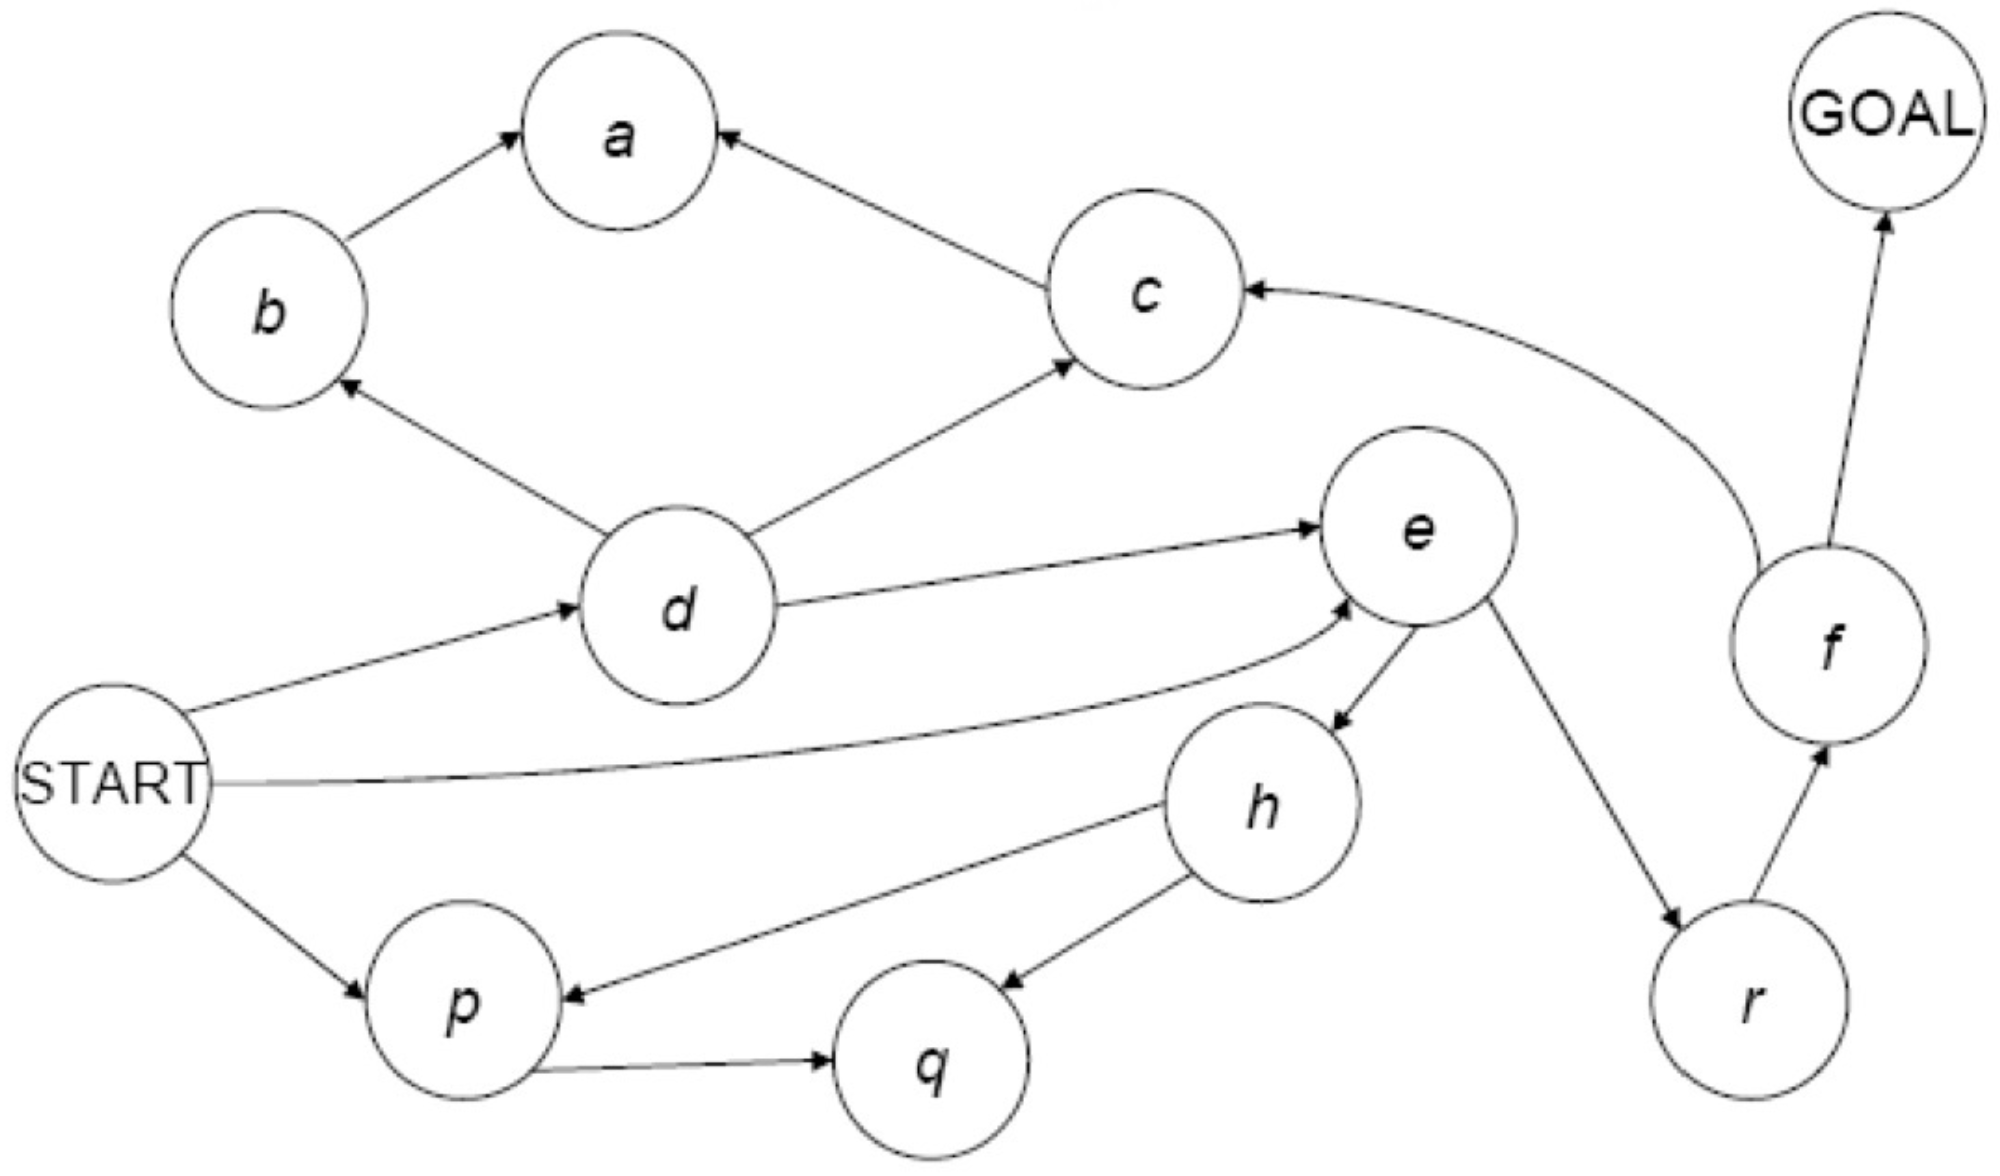
\includegraphics[width=0.45\linewidth]{figures/Search Graph Rep.png}
    \end{center}

    which yields the search tree

    \begin{center}
        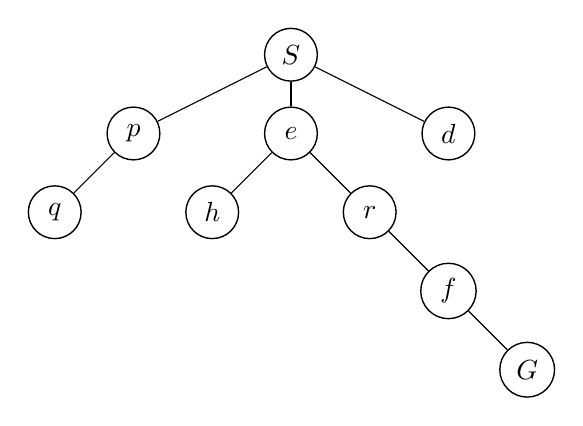
\begin{tikzpicture}[ tree-node/.style={ circle, draw=black, line width=0.5pt, minimum size=0.67cm, } ]
            \node[tree-node] (S) at (0, 0) {$S$};
            \node[tree-node] (P) at (-2, -1) {$p$};
            \node[tree-node] (E) at (0, -1) {$e$};
            \node[tree-node] (D) at (2, -1) {$d$};
            \node[tree-node] (Q) at (-3, -2) {$q$};
            \node[tree-node] (H) at (-1, -2) {$h$};
            \node[tree-node] (R) at (1, -2) {$r$};
            \node[tree-node] (F) at (2, -3) {$f$};
            \node[tree-node] (G) at (3, -4) {$G$};

            % Edges
            \draw (S) -- (P);
            \draw (S) -- (E);
            \draw (S) -- (D);
            \draw (P) -- (Q);
            \draw (E) -- (H);
            \draw (E) -- (R);
            \draw (R) -- (F);
            \draw (F) -- (G);
        \end{tikzpicture}
    \end{center}
\end{example}

\begin{listu}
    \item \textbf{Completeness}
    
    \begin{listu}
        \item BFS is \term{complete} if the \bred{branching factor} is \itblue{finite}.
        \item The length of the path (from the initial node to the node removed from the \Frontier) is \itblue{non-decreasing}, as we replace eac expanded node with path langth $k$ with a node with path length of $k + 1$. 
    \end{listu}

    \item \textbf{Optimality}
    
    \begin{listu}
        \item BFS gives the \bred{shortest length solution}. 

        All nodes with shorter paths are expanded prior to any node with longer path. We examine all paths of length $< k$ before all paths of length $k$. Thus, if there is a solution with length $k$, we will find it before longer solutions. 

        \item BFS is \bred{not} optimal in terms of \itblue{cost}.
        
        BFS does not take into account the cost of the path. It is possible that a longer path has a lower cost than a shorter path.
    \end{listu}
\end{listu}

% TODO: Romnia Travel Example, see slides page 35

\subsubsection{Properties of BFS}

Let $b$ be the maximum branching factor and $d$ be the depth of the shallowest goal node.

\begin{listu}
    \item \textbf{Time Complexity} \[
        1 + b + b^2 + \cdots + b^d + b(b^d - 1) \in O(b^{d+1})
    \]

    The last term id $b(b^d - 1)$ because we need to remove the goal node, who does not need any successors.

    \item \textbf{Space Complexity} \[
        \mathcal{O}(b^{d+1})
    \]
    
    In the worst case, only the last node of depth $d$ satisfies the goal. So all nodes at depth $d$ except the last one will be expanded by the search and each such expansion will add up to $b$ new nodes to the \Frontier.
\end{listu}

\begin{table}[ht!]
    \renewcommand{\arraystretch}{1.25}
    \centering
    \begin{tabular}{| l | l | l | l |}
        \hline
        Depth & Paths    & Time          & Memory    \\ \hline
        1     & $1$      & 0.01 millisec & 100 bytes \\ \hline
        6     & $10^6$   & 10 sec.       & 100 MB    \\ \hline
        8     & $10^8$   & 17 min.       & 10 GB     \\ \hline
        9     & $10^{9}$ & 3 hrs.        & 100 GB    \\ \hline
    \end{tabular}
\end{table}

Space complexity is a bigger problem than time complexity. Typically, BFS rus out of memory before it runs out of time.

\subsection{Depth-First Search}

\begin{definition}[Depth-First Search]\label{def:dfs}
    \term{Depth-First Search} is a search strategy that expands the deepest unexpanded node first.
\end{definition}

DFS explores the search tree \itblue{branch by branch}. It place the children of the current node at the \bred{front} of the \Frontier. This means the \Frontier is a \bred{stack}, and we always extract the \itblue{first} element from the \Frontier.